\documentclass[fleqn]{article}
\oddsidemargin 0.0in
\textwidth 6.0in
\thispagestyle{empty}
\usepackage{import}
\usepackage{amsmath}
\usepackage{graphicx}
\usepackage{flexisym}
\usepackage{amssymb}
\usepackage{bigints} 
\usepackage[english]{babel}
\usepackage[utf8x]{inputenc}
\usepackage{float}
\usepackage[colorinlistoftodos]{todonotes}

\definecolor{hwColor}{HTML}{AD53BA}

\begin{document}

  \begin{titlepage}

    \newcommand{\HRule}{\rule{\linewidth}{0.5mm}}

    \center


    \textsc{\LARGE Arizona State University}\\[1.5cm]

    \textsc{\LARGE Mathematical Methods For Physics II }\\[1.5cm]


    \begin{figure}
      
\includegraphics[width=\linewidth]{asu.png}
    \end{figure}


    \HRule \\[0.4cm]
    { \huge \bfseries Homework Six}\\[0.4cm] 
    \HRule \\[1.5cm]

    \textbf{Behnam Amiri}

    \bigbreak

    \textbf{Prof: Cecilia Lunardini}

    \bigbreak


    \textbf{{\large \today}\\[2cm]}

    \vfill

  \end{titlepage}


  \textbf{Part A}
  \begin{enumerate}
    \item  Derive the expression for the Dirac Delta in spherical polar coordinates (see lecture for a similar example): 
      $$
      \delta^{(3)}(\mathbf{r}-\mathbf{r_0})=\frac{1}{r^2} \delta(r - r_0) \delta(\cos \theta - \cos \theta_0) \delta(\phi - \phi_0).
      $$
    Here $\mathbf{r}$ is the position vector and $r=|\mathbf{r}|$. The symbols with the 0 subscript refer to a fixed point in space. 

    \item  Use the Heaviside step function to write the function: 
      $$
      f(x)= 
      \begin{cases}
      0 ~~{\rm  if}~x<-\pi \\
      \cos x ~~{\rm  if}~-\pi<x<\pi \\
      0 ~~{\rm  if}~x>\pi0 \\
      
      \end{cases}
      $$
    as a single expression.  


    \item prove that the derivative of the Dirac Delta is odd, in other words: $\delta^\prime(-x)=-\delta^\prime(x)$. 
  \end{enumerate}

  \textbf{Part B}
  \begin{enumerate}
    \item The table below shows some useful Fourier Transforms of common functions. For each case the function $f(x)$ is given (second column of the table) along with its graph (first column). The third column gives  $g(k) \sqrt{2 \pi}$, where $g(k)={ \mathcal F(f)}$. 
    \begin{figure}[h]
      \begin{center}
        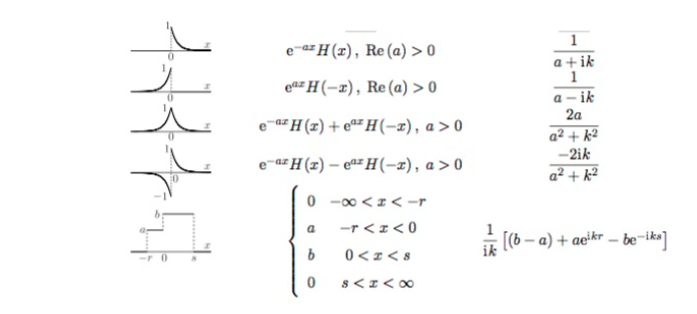
\includegraphics[width=0.7\textwidth]{usefulTable.PNG}
      \end{center}
    \end{figure}

    using this table, find the inverse Fourier Transform  of the following functions:
    \begin{enumerate}
      \item $g(k) = \frac{1}{\sqrt{2\pi}} \frac{e^{-(3 + ik)}}{3 + ik}$

      \item $g(k)=\frac{1}{\sqrt{2\pi}}\frac{1}{2 + i(k-1)}$

      \item $g(k)=\frac{1}{\sqrt{2\pi}}\frac{ik}{(1+ik)(2 + ik)}$

    \end{enumerate}



    \item  Use the convolution theorem to solve the following integral equation (in other words, find $y(t)$): 
      $$
      y(t)=r(t) + \int_{-\infty}^{+\infty} y(x) r(t - x) dx. 
      $$
    where $r(t)=e^{-3|t|}$. \\
    (Hint: start by taking the Fourier Transform of each side of the equation. )
  \end{enumerate}

\end{document}
